\documentclass[a4paper,12pt]{report}
\usepackage[hmargin=1in, vmargin=1in]{geometry}
\usepackage[shortlabels,inline]{enumitem}
\usepackage{amsmath, amssymb, array, booktabs, multicol, multirow, setspace, hyperref, graphicx}
\usepackage[labelfont=bf]{caption}

\hypersetup{
    colorlinks,
    citecolor=black,
    filecolor=black,
    linkcolor=black,
    urlcolor=blacks
}

\newcommand{\msection}[1]{\noindent\textbf{#1}}
% \doublespacing
\newcommand{\authorname}[3]{
    \begin{minipage}[t]{.25\linewidth}
        \centering
        \textbf{#1} \\
        \small #2 \\
        #3
    \end{minipage}
}

\newenvironment{bottom}{\par\vspace*{\fill}}{\clearpage}

\begin{document}

\begin{titlepage}
    \centering
    \large Assignment \#4 
    \vspace*{.4in}

    \vspace*{.25in}
    \Large\textbf{Group 20: Everglades Analytics Design Document}
    \normalsize
    \vspace*{.25in}
    
    % First name alphabetical order 
    % Elaine Ng, Ian Pleau, Manuel Vasquez, Ossama Amer, Thomas Lukas
    
    \authorname{Elaine Ng}{Computer Science (BS)}{Statistics (BS)}
    \authorname{Ian Pleau}{Computer Science (BS)}{}
    \authorname{Manuel Vasquez}{Computer Science (BS)}{Statistics Minor}
    \vspace*{.125in}
    
    \authorname{Ossama Amer}{Computer Science (BS)}{}
    \authorname{Thomas Lukas}{Computer Science (BS)}{SCAN Minor}
    
    \vspace*{.25in}
    \today
    
    \vspace*{.4in}
    \noindent\rule{.5\linewidth}{.4pt}
    \vspace*{.4in}

    % flushes logos to bottom
    % \begin{bottom}
        \begin{minipage}[c]{.35\linewidth}
            \centering
            
\includegraphics[width=1\linewidth]{media/lm.png}
        \end{minipage}
        \begin{minipage}[c]{.3\linewidth}
            \centering
            
\includegraphics[width=.2\linewidth]{media/ucf.png}
        \end{minipage}
    % \end{bottom}
\end{titlepage}

\onehalfspacing
\pagenumbering{roman}

\tableofcontents

\newpage

\setlength{\parskip}{\baselineskip}
\setlength{\parindent}{0in}
\pagenumbering{arabic}

\chapter{Executive Summary}
\section{Goals and Objectives}

\chapter{Technical Content}
\section{Project Overview}

The Everglades Agent Behavior Analytics project is a project with the goal to set the baseline for accurate analysis of RTS (Real-Time Strategy) data that is used to learn and infer better strategies for the future. The origin of the use of this analysis is the Everglades RTS game that Lockheed Martin has developed and is being worked on by another team. Due to the current lack of meaningful data, it was important to focus on a similar RTS to get meaningful data and that is where StarCraft comes in. StarCraft as a game is a very complex real-time strategy game, it features three primary archetypes or races to play as, Zerg, Terran, or Protoss, within these races it has thousands of different strategies and ways to play the game and therefore has received a massive following over its long tenure as a popular game. With its massive popularity comes a large data set that is out there known as StarData through this it is possible to completely analyze over 60,000 games of StarCraft data for use.

Everglades as an RTS game has the goals of having specific unit compositions, strategies, base layouts, and more all features that are present in StarCraft which makes it the perfect Game for effective crossover data. The current overarching goal of the project is to utilize statistics, supervised learning, and unsupervised learning to study Behaviors that Lead to Wins, Losses, and other major events that can occur within the StarCraft game. The starting Objectives will be to use the database of info and start setting up some initial learning patterns given the data to focus on Wins and Losses. As the project progresses smaller objectives such as unit compositions will become an objective with setting up algorithms that make these possible.  The function of gathering all this data is overall to have a good basis for further gathering and development of data. With this starting point once the Everglades project has data that is needing to be analyzed the methodology and tools are already developed and ready to go and only need slight changes to switch from being a StarCraft data set to the everglades data.

\section{Personal Motivations}

\msection{Elaine Ng}

When I first heard the Everglades’ project pitch, I was immediately interested because it was a strategy video game. Then the different teams for the project were presented and I saw that there was going to be an Analytics Team. I knew at that moment that the Everglades: Robot Behavior Analytics Team was the perfect senior design project for me. As someone who spends a lot of time playing video games and is also currently studying for a Computer Science and Statistics degree, I felt that this project brought many of my passions together. Having the opportunity to learn how to gather, analyze, and predict for large video game data sets with a dedicated team and knowledgeable guidance is definitely one of my main motivations for the Everglades project. This will be one of my largest projects yet, and I am very excited to be a part of this.

\msection{Ian Pleau}

The everglades projects were presented by Lockheed all in one go and immediately they all ranked highly on my list of preferred projects. The idea of working on a real-time strategy(RTS) type project and having the opportunity to either work on the game side of the database and analytics side piqued my interest. Ultimately, I leaned more towards the analytics side choosing that as my first choice. My reasoning for this choice was that I always in the past had been heavily focused on numbers and data when looking to optimize in games, programming, or even just decisions I would make in day to day life. The project was initially proposed with the possibility of working with Everglades data but also working with StarCraft data to create a baseline idea for how to analyze a win rate and a real-time strategy data set.

\msection{Manuel Vasquez}

I think I’m in the wrong major. When I began university I just wanted to learn how to code, but as I progressed through my courses I realized that I’m actually more interested in gathering insights from otherwise obscure data. This project is giving me the opportunity to acquire real-life skills and learn how to present my findings to professionals in other fields. The club AI@UCF introduced me to the basics of many libraries like Tensorflow, Torch, and Sci-kit learn. UCF taught how to find statistically relevant information from simple datasets. Now I’m able to merge these two knowledge bases into what we’re calling Everglades Analytics.

I’ve attended enough lectures about reinforcement learning to know that I have no idea what I’m doing. Thankfully, this project focuses on the analytics aspect of the Everglades project. Novel models like AlphaStar have greatly advanced the area of reinforcement learning. With many research papers discussing the developers’ ground-breaking approaches and the model’s super-human performance on several real-time strategy games. Given AlphaStar’s almost perfect approach to Starcraft, we can study this model and possibly discover actionably better strategies than our current STARDATA dataset can provide.

\msection{Ossama Amer}

Due to my interest in Data Science, I was ecstatic to participate in this project. Acquiring analytics from a real-time military science game in order to match output to attain the most wins is something I feel I can greatly benefit from as a computer science student. We look forward to making our sponsors proud and more importantly, delivering efficient results, further bettering the EVERGLADES project through artificial intelligence advancement. Aside from the project, I also look forward to networking with my teammates and developing new connections while discovering new technologies.

\msection{Thomas Lukas}

When the initial project was presented, I was immediately hooked with the idea of a strategy game that can be used as a foundation to teach the process of creating and training AI. Strategy board games and video games have always been a big part of my life growing up, I always tried my hardest to discover and sometimes attempt to create a new “meta” that can balance the odds in my favor. Working with StarCraft data, I am more than excited to see the mathematical representation that each “meta” strategy implemented by the factions will look like in the grand scheme of things. I am eagerly looking forward to getting the results and seeing what strategies could be potentially translated to the EVERGLADES project for future teams in senior design around the nation.

\section{Broader Impacts}

The "broader impact" of this project is to set up a baseline for further research into successful strategies for RTS games, specifically applying this to the everglades project. With the everglades project acting as an RTS training simulator for the strategy of drones, the information and statistics of the unit management and efficiency could become a stepping stone for further research and real-life application. Talking specifically about Lockheed as a military contractor data analysis of drone strategies could eventually lead to enhancements in defense combat or national security and then broader a look into how to manage a fleet of drones efficiently for non-combat uses. Non-combat drone usage could be wide from non-profit work and environmental work to enhanced infrastructure and improvements to the way companies view shipping.

\section{Legal, Ethical, and Privacy Issues}

Legally the work within Data analysis for StarCraft and Everglades is not under NDA. This however does not mean the project is open source and information regarding the sharing and distribution of the programs and analysis that is produced is decided by the sponsor Lockheed Martin. Ethically because we are working with StarCraft data it is hard to say that anything is questionable and there were no problems encountered within it going forward the use of the analysis could be used for efforts that are not as ethical but as of now it is a non-issue. Privacy Issues have also not been a problem nor are they likely to pop up in future use of the implementation.

\section{Project Requirements and Specifications}

\subsection{Goal \#1}

\textit{Characterize StarCraft match output from a publicly available dataset to determine behaviors that most often lead to wins.}

\textbf{Description |} StarCraft match output data sets would be analyzed to identify characteristics. Characteristics that are statistically significant in determining the win rate would be clearly documented and be used for the other goals in predicting match outcomes. Characteristics that are not statistically significant in determining win rate will not be considered for behaviors that most often lead to wins but will still be recorded for the reason that it might help increase the accuracy of match outcome prediction.

\textbf{Specifications |} We suggest that for this goal we should find at least 5 characteristics that are statistically significant in determining the win rate. Optimistically, we would be able to identify more winning behaviors, as well as filter out the statistically insignificant characteristics that we might have identified during the process. 

\subsection{Goal \#2}

\textit{Propose new metrics to predict agent performance, similar to Sabermetrics.}

\textbf{Description |} Research should be done on StarCraft and data sets should be analyzed in order to find new metrics that are statistically significant in predicting agent performance and their match outcomes. Such as, but not limited to, action per minute (APM), damage per second (DPS), strategies used, micro and macro.

\textbf{Specifications |} We suggest that for this goal we should find at least 5 new metrics that are statistically significant in predicting agent performance. Optimistically, we would be able to propose more metrics that can be utilized to predict agent performance. We hope that with these newly proposed metrics, we are able to predict outcomes more accurately and demonstrate the reasons behind agents’ match outcomes. 

\subsection{Goal \#3}

\textit{Identify how map differences affect the output of games with similar strategies.}

\textbf{Description |} Research should be done on StarCraft maps and the types of strategies. The differences between maps and the types of strategies available on StarCraft should be identified. The map differences that are statistically significant in affecting game outputs with similar strategies will be clearly documented.

\textbf{Specifications |} We suggest that for this goal we should find at least 3 map characteristics that are statistically significant in affecting the output of games with similar strategies. Optimistically, we would be able to find more map differences that have an effect on game output and be able to show which strategy works best for the different types of maps.

\subsection{Goal \#4}

\textit{Implement a supervised machine learning classification algorithm that predicts the outcome of a match given the current game state.}

\textbf{Description |} We would build a software analysis tool that can take in the specific details of the match and correctly have a successful prediction of future game results. Using the previous must-have requirements, the algorithm should be able to use those metrics to accurately predict which player is expected to come out victorious.

\textbf{Specifications |} We suggest that this algorithm should have above a 75\% accuracy when predicting after the early game, early game predictions in StarCraft can easily fluctuate based on human player blunders and strategy implementation. The stretch end goal is to produce an algorithm that can predict with high accuracy at any point in the match.

\subsection{Goal \#5}

\textit{Develop a real-time analytics engine that runs simultaneously with StarCraft match playback. The engine should be at a minimum to predict odds of winning and describe the agent behaviors.}

\textbf{Description |} The home run goal of the entire project is to create a real-time predictor, similar to something you would see in a poker match on TV. In those poker games, the hand odds are calculated and predicted win probabilities are given to each player competing in the current hand shown in real-time. Similarly, the software program we would develop would take in the metrics provided in the goals above and output a real-time predicted win probability every five seconds or so.

\textbf{Specifications |} We suggest that this algorithm should have a plausible enough accuracy at every point of the game. Similar to the stretch goal above, after the early game the algorithm should have above a 75\% accuracy of predicting the correct outcome. Starting from early game strategies and economies, the predictor should never give a player a near 100\% accuracy to win right before they blunder and lose the game. Although human error may always provide outliers, this should not be an excuse for the predictor on average to have a below-average prediction accuracy.  

\section{Possible Features}

\msection{Elaine Ng}

We could go into a more statistical direction and use regression analysis to attempt to find the relationships between certain variables/characteristics in regards to winning rate, agent performance, and map differences, and the type of strategy used. Perhaps a logistic regression is a good place to start since we are dealing with a categorical dependent variable (win or lose). We can also try to use machine learning methods to predict performance such as supervised or unsupervised learning.

\msection{Ian Pleau}

Going in a research-based direction could be extremely beneficial for this project. This means reading as many papers to get ideas of how we are going to analyze and structure data from StarCraft as possible before going into the data analysis. Starcraft has a lot of statistics that lead to a win or a loss, the key will be to identify which of these stats are the best possible for us to deep analyze. Shoehorning off of Thomas one of the best statistics that could be looked at is definitely the different races and what they mean for playstyle, game times, and win rates at specified moments of the game. This could open a bigger analysis into studying spikes in win rate over time, does minute 30 of a game have a large win rate spike in a certain race because they are able to achieve a powerful unit at that time or other analysis.

\msection{Manuel Vasquez}

To start off the project we should do exploratory data analysis. To gain a deeper understanding of what simple strategies utilized by players we can perform clustering. Applying K-means can render useful results. To continue with the issue of strategy, we could classify approaches by build order (STARDATA. 2017). This can even provide insight into troop usage and the rate of resources mined. This approach would not tell us which strategy is best, since there are other influential factors that also need to be observed, e.g.: warfare handling and enemy status prediction.

\msection{Ossama Amer}

Expanding on Elaine’s idea of delving into a more statistical direction, I think we should also use correlation analysis to explore the relationships between the behaviors and outcomes. Identifying if data is symmetrical and interchangeable is key to verifying if we are acquiring the expected outcomes. If we can pick up on certain actions and behaviors being correlated with wins or losses, that will allow us to dive deeper into the idea of regression analysis and see exactly what causes those outcomes, that way we can modify algorithms accordingly.

\msection{Thomas Lukas}

Initial building and unit decisions are among the most important parts of the game, especially if one of the races in the match is Zerg. Zerg players tend to be overly aggressive in their unit creation and attack tactics so if the opposing player does not implement the correct counter strategy, the Zerg player will snowball into a victory. We believe that if our algorithm can identify the early strategies of both players it can accurately predict a quick win depending on if a player is getting countered perfectly. One problem that can arise however is that since this will be human vs human matches, there is always the chance for the player with the superior strategy to blunder in execution and lose the game.

\section{Distribution of Work}

\section{Project Block Diagram}
\begin{center}
    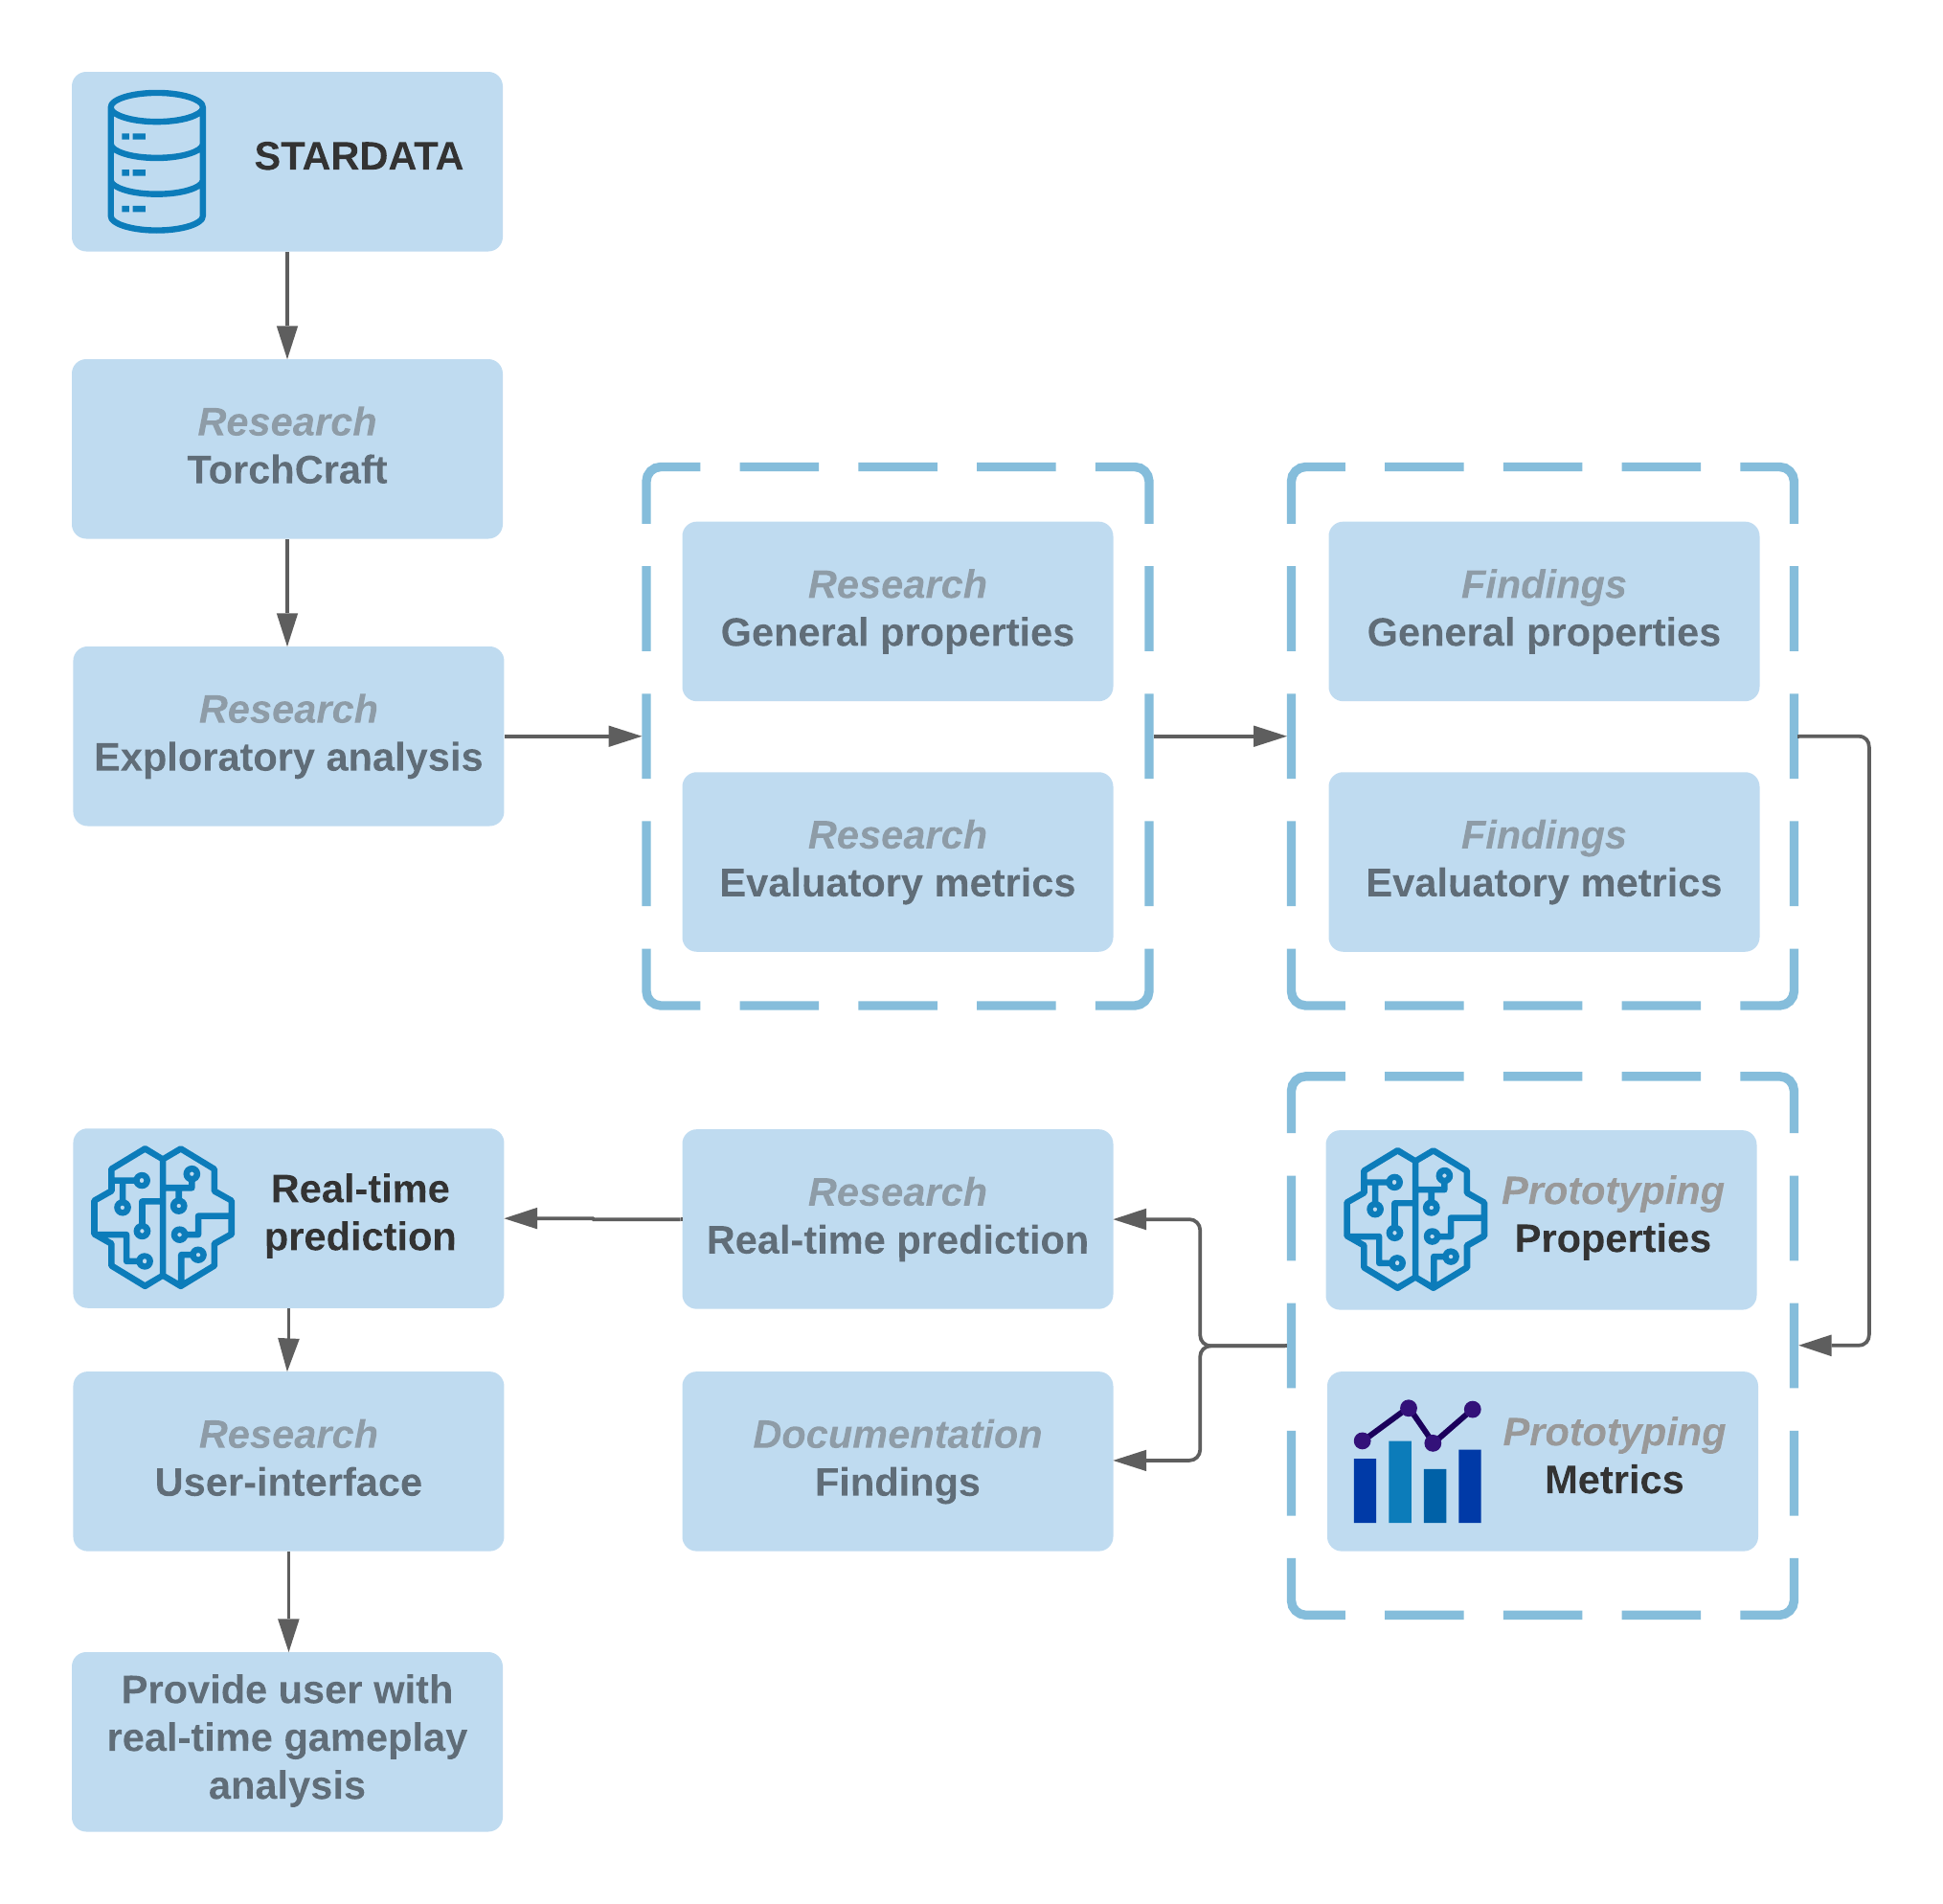
\includegraphics[width=.9\linewidth]{media/block_diagram.png}
    
    % just ignore its whinning
    % tHe OpTiOn `hYcAp=TrUe` wIlL bE iGnOrEd
    \captionof{figure}{Working project block diagram as of September 30, 2020.}
\end{center}

\chapter{Research}
\section{Game Mechanics}
\subsection{Subsections explaining mechanics}
\section{Data Exploration}
\section{Supervised Learning}
\section{Unsupervised Learning}
\section{Model Methodologies}
\section{Real-world Applications}

\chapter{Design}
\section{Model Trainining}
\subsection{Subsections explaining what we did}
\section{Model Validation}
\subsection{Subsections explaining what we did}
\section{Database}
\subsection{Subsections explaining what we did}

\chapter{Administrative Content}
\section{Project Budget}

Aside from testing the agents through a server, there are no expected costs for the duration of this project. The server will be implemented through Amazon Web Services (AWS) or Microsoft Azure which will yield no further than \$100.

Upon completion of the project, the remaining costs obtained from the group will involve printing, binding, and documentation near the end of Senior Design I. These costs may vary depending on a few possible options pertaining to the color and size of the documentation.

\section{Project Milestones}

\subsection{Initial Research and Analysis}

The team will be acclimating to several different technologies ranging from Scikit-learn, Python, and TensorFlow. Scikit-learn is a Python-based machine learning tool that enables the diagnosis of large datasets while also providing a visual representation of the corresponding data. TensorFlow is an open-source software library for dataflow for machine learning applications. Alongside the technologies, we will also be diving into StarCraft, Brood War extension pack, a military science real-time strategy game offered by Blizzard Entertainment. The team would be learning the functionalities of the game as the goal is to characterize match output from a publicly available dataset to determine behaviors most often leading to wins. Deliverables will be produced from what the team explored during the research of StarCraft data machine learning concepts.

\subsection{Agile Sprints}

Throughout this project, we will be required to attain AI agents and their variable metrics. To do so, the team will work through the development process using Agile Sprints. Each sprint will consist of Hypothesis Generation/Data Preparation, AI Agent Development, Agent Testing/Comparison, and Final Data Review.

\subsection{Data preparation}

Preparation of data includes but is not limited to research and analysis through StarCraft dataset, learning machine learning concepts through StarCraft’s Brood War expansion pack, reinforcement learning, and generative models.

\begin{center}\begin{tabular}{ll}
Sprint 1 & 10/19/2020 \\
Sprint 2 & 11/12/2020 \\
Sprint 3 & 01/20/2021
\end{tabular}\end{center}

\subsection{Agent Testing/Comparison}

Agent testing and comparison will be handled once the team acquires a hypothesis regarding the relevant metrics causing and affecting certain behaviors and outcomes. These methods include but are not limited to identifying early game strategies, using regression analysis, and correlation analysis.


\begin{center}\begin{tabular}{ll}
Sprint 1 & 10/24/2020 \\
Sprint 2 & 12/02/2020 \\
Sprint 3 & 02/05/2021
\end{tabular}\end{center}

\subsection{Data review and revision}

The number of models and prototypes developed from the team will provide a sufficient reason as to what causes agents/players to achieve victories. The team is aiming for the simplification of the technical information therefore, portions of the data will be molded into a non-technical review as far as the artificial intelligence is taken place within the real-time strategy military game.

\begin{center}\begin{tabular}{ll}
Sprint 1 & 10/31/2020 \\
Sprint 2 & 12/10/2020 \\
Sprint 3 & 02/11/2021
\end{tabular}\end{center}

\subsection{Final Design Document}

Following through with the final design documentation will require juxtaposition from several distinct platforms including but not limited to Jira, Trello, TensorFlow, and GitHub. Constructing a clear, concise, and coherent document is the goal in which all team-members will cooperate.

\chapter{Conclusions \& Future Work}
\chapter{References}
\chapter{Appendix}

\end{document}